\documentclass[11pt]{article}
\usepackage[utf8]{inputenc}
\usepackage[T1]{fontenc}
\usepackage[spanish,es-nodecimaldot]{babel}
\usepackage[a4paper,margin=2.4cm]{geometry}
\usepackage{amsmath,amssymb,booktabs,graphicx,siunitx,tabularx,url,microtype}
\usepackage{url}
\sisetup{output-decimal-marker={,},group-separator={.},per-mode=symbol}
\setlength{\parindent}{1em}
\setlength{\parskip}{0.18em}
\setlength{\textfloatsep}{3pt}
\setlength{\intextsep}{3pt}
\setlength{\floatsep}{3pt}
\setlength{\abovecaptionskip}{2pt}
\setlength{\belowcaptionskip}{1pt}
\title{Test 1 -- Malla, error de campo y condiciones de borde}
\author{Luis Angel Broncano Marcelo\\Ingeniería Civil en Obras Civiles -- USACH}
\date{5 de noviembre de 2026}

\begin{document}
\maketitle
\vspace{-1.0em}

\section{Problema y referencia independiente}
Se estudia una barra axial lineal elástica con $L=2000\,\mathrm{mm}$, $E=200000\,\mathrm{N/mm^2}$, $A=1000\,\mathrm{mm^2}$, $P=20000\,\mathrm{N}$ y $q=10\,\mathrm{N/mm}$, ambos hacia $+x$. El contorno base es $u(0)=0$ y $EAu'(L)=P$. Con $E,A$ constantes, $-(EAu')'=q$; integrando se obtiene la referencia
\[
 u_{\mathrm{ref}}(x)=\frac{Px+q(Lx-x^2/2)}{EA},\qquad
 u_{\mathrm{ref}}(L)=0{,}300000\,\mathrm{mm}.
\]
El modelo y su formulación axial corresponden al planteamiento de barra indicado en el material de consulta \cite{tudelftrod}. Se conservó el solver NumPy suministrado, que resuelve el sistema lineal reducido \cite{numpy}.

\section{Predicción y método}
Antes de ejecutar, se predijo que el campo MEF lineal coincidiría con la referencia en los nodos, pero no entre ellos. La interpolación lineal de la solución cuadrática produce en el punto medio de cada elemento un error máximo $\varepsilon_{m}=qh^2/(8EA)$; al duplicar $n$, $h=L/n$ se reduce a la mitad y el error a la cuarta parte. En \texttt{src/analisis.py} se implementaron la referencia y la evaluación del error usando el promedio de desplazamientos nodales adyacentes. En \texttt{src/ejecutar.py} se añadieron el balance relativo, el residuo libre, las salidas CSV y las figuras; \texttt{src/barra\_mef.py} no se modificó.

\section{Resultados y verificación}
\begin{center}
\setlength{\tabcolsep}{3pt}
\begin{tabular}{rrrrrrrr}
\toprule
Caso & $n$ & $h$ [mm] & $u(L)$ [mm] & $R_0$ [N] & $R_L$ [N] & $\varepsilon_m$ [mm] & $\eta_{bal}$ \\
\midrule
Base & 2 & 1000 & 0,300000 & $-40000$ & $\approx0$ & 0,006250 & $0$ \\
Base & 4 & 500 & 0,300000 & $-40000$ & $\approx0$ & 0,0015625 & $5,46\times10^{-16}$ \\
Base & 8 & 250 & 0,300000 & $-40000$ & $\approx0$ & 0,000390625 & $9,10\times10^{-16}$ \\
$u(L)=0$ & 8 & 250 & 0 & $-10000$ & $-30000$ & -- & $0$ \\
\bottomrule
\end{tabular}
\end{center}
En el contorno base, los desplazamientos nodales coinciden con $u_{\mathrm{ref}}$; por tanto, el acuerdo nodal no acredita por sí solo la exactitud del campo interpolado. Los errores calculados en puntos medios coinciden con $qh^2/(8EA)$ y siguen la tendencia $n^{-2}$. El residuo $r=Ku-f$ es menor o igual que $5{,}82\times10^{-11}\,\mathrm{N}$ en los grados libres; allí se verifica el equilibrio de las ecuaciones. En los grados restringidos aparecen las reacciones. Con $K$ y $f$ originales, el máximo balance relativo $|\sum R+P+qL|/|P+qL|$ fue $9{,}10\times10^{-16}$, menor que $10^{-8}$. Esta tolerancia es un control de consistencia numérica, no una validación física experimental.

\begin{figure}[ht]
\centering
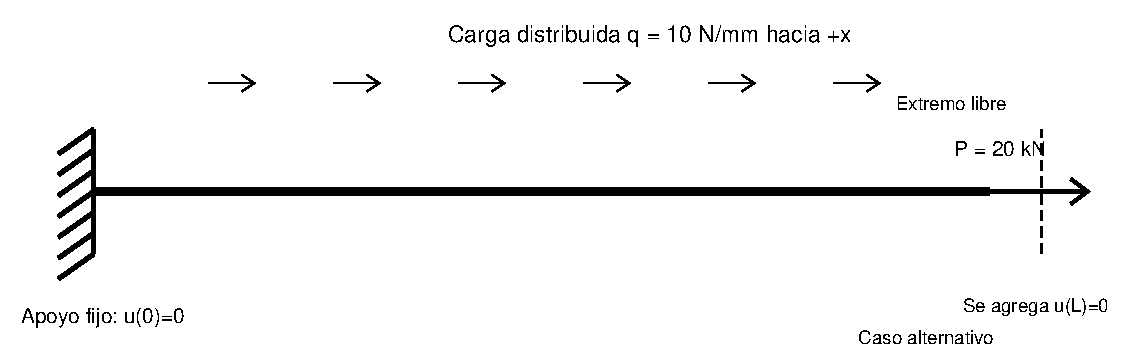
\includegraphics[width=0.80\linewidth]{figures/contorno.pdf}
\caption{Contorno original y restricción adicional del caso alternativo.}
\end{figure}
\begin{figure}[ht]
\centering
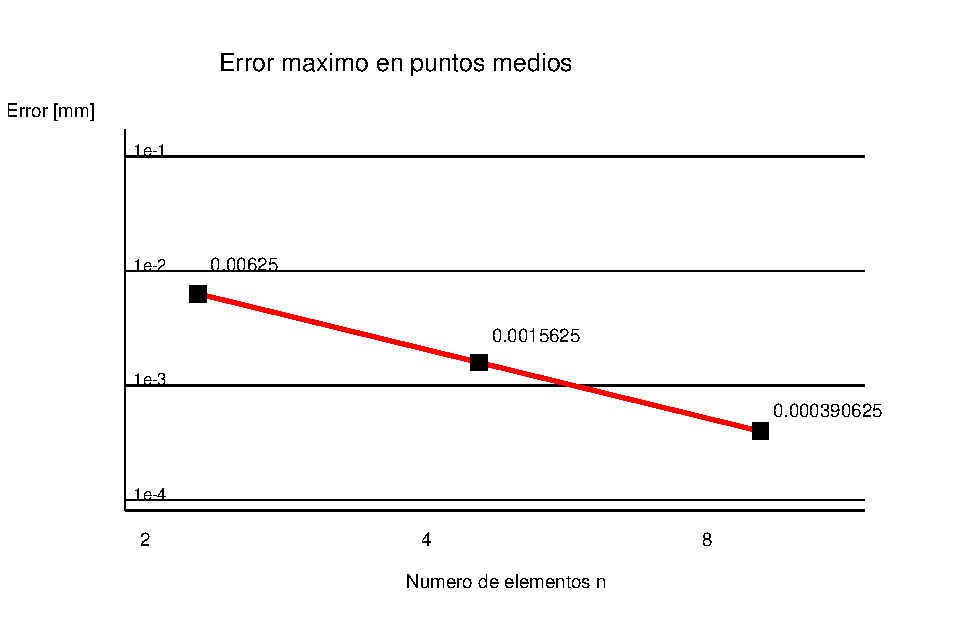
\includegraphics[width=0.62\linewidth]{figures/convergencia.pdf}
\caption{Error máximo en puntos medios frente al número de elementos.}
\end{figure}

\section{Cambio de contorno e interpretación}
Al imponer además $u(L)=0$ se resuelve otro problema de borde, aunque las cargas se mantengan. Para $n=8$, $u(L)$ cambia de $0{,}300000$ a $0\,\mathrm{mm}$; en $x=1000\,\mathrm{mm}$, el desplazamiento cambia de $0{,}175$ a $0{,}025\,\mathrm{mm}$. La nueva restricción genera $R_0=-10000\,\mathrm{N}$ y $R_L=-30000\,\mathrm{N}$. El balance también cierra porque las reacciones del sistema restringido equilibran las cargas aplicadas; esto verifica equilibrio estático, no que se haya conservado el contorno original.

\textbf{Conclusión.} El refinamiento no cambió los desplazamientos nodales, que ya coinciden con la referencia, pero redujo el error entre nodos como $h^2$. Por ello, el acuerdo nodal no basta para aceptar todo el campo aproximado. Agregar $u(L)=0$ cambió el problema: anuló el desplazamiento del extremo y redistribuyó las reacciones. El cierre del equilibrio en ambos casos no demuestra que sus condiciones de borde sean equivalentes.

\textbf{Trazabilidad y uso de IA.} Se ejecutó \texttt{python -m pytest -q} (5 pruebas aprobadas) y \texttt{python src/ejecutar.py}. Los datos están en \texttt{salidas/resultados.csv} y \texttt{salidas/desplazamientos\_nodales.csv}; versiones y registros, en \texttt{salidas/versiones.txt} y \texttt{registros/}. Se usó ChatGPT para apoyar la derivación, implementación de funciones pendientes y redacción; los resultados se contrastaron con la referencia analítica y las pruebas. El estudiante debe verificar y poder explicar el contenido. No se ejecutó MAPDL.

\bibliographystyle{plain}
\bibliography{referencias}
\end{document}
